\section{Flat shoulders and the convex fit}\label{sec:mechanism}

This section proves that the uniform calibration fails, and shows where the law of $M$ enters. The argument has three ingredients: an exact formula for the convex distance, a condition that forces the fit to be convex on a stretch of the data, and the Brownian limit of the empirical process on that stretch.

\subsection{The picture}
Write $W(w,\varepsilon)$ for the two-step law on $[0,1]$ whose density equals $(1-w)/(1-\varepsilon)$ on $(0,1-\varepsilon)$ and $w/\varepsilon$ on $(1-\varepsilon,1)$, with $0<\varepsilon<w<1$. The long flat part carries mass $1-w$; we call it the \emph{shoulder}. The short interval at the right end carries mass $w$ and has a much higher density; we call it the \emph{top}. The law in \cref{fig:fixedlaw} is $W(0.1,0.005)$, and we use it as a running example. \Cref{fig:mechanism}(a) shows the shape.

\begin{figure}[t]
\centering
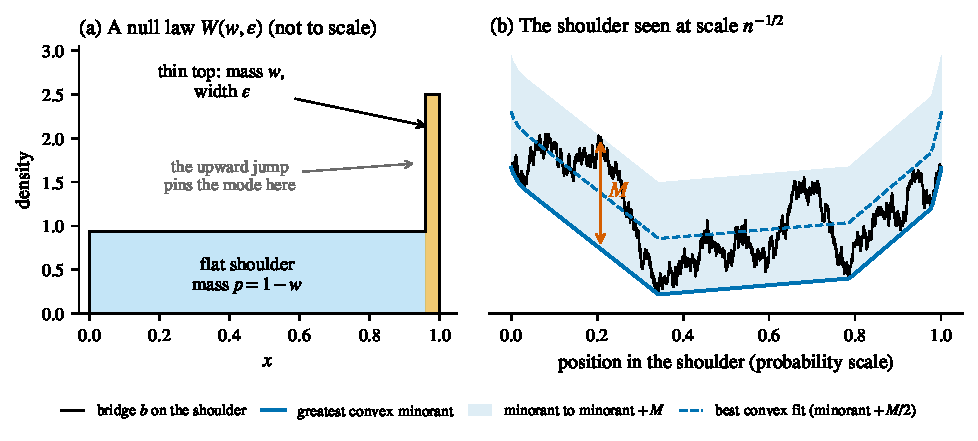
\includegraphics[width=\linewidth]{figs/fig1_mechanism.pdf}
\caption{A pinned shoulder forces the fit to curve upward over the whole shoulder, and the best such fit to a Brownian bridge misses it by half the largest gap $M$. (a) The null law $W(w,\varepsilon)$: a flat shoulder of mass $1-w$ followed by a thin top. Because the density jumps up at the start of the top, every close unimodal fit must turn to the right of any fixed point inside the shoulder, so the fit is convex there. (b) After removing its chord and rescaling, $\sqrt n(F_n-F)$ on the shoulder is close in law to $\sqrt{1-w}$ times a Brownian bridge; one simulated bridge $b$ is shown. A convex function within distance $d$ of $b$ lies below the greatest convex minorant plus $d$, so it cannot reach the top of the largest gap $M$ unless $d\ge M/2$. The minorant shifted up by $M/2$ (dashed) attains this. Under the uniform law the fit may turn anywhere, which gives the smaller limit $D(B)$.}
\label{fig:mechanism}
\end{figure}

Imagine fitting a unimodal distribution function to a large sample from $W(0.1,0.005)$. The true distribution function rises slowly along the shoulder and then very steeply over the top. A good fit must follow that steep rise, so it must still be rising steeply at $0.995$; a unimodal distribution function rises fastest at its mode, so the fit's turning point has to sit in the top. Over the whole shoulder, then, the fit is on the convex side of its turning point. It cannot bend the other way to follow a random bump in the data, as it could under the uniform law. On the shoulder the dip is therefore at least the convex distance of the data, and the next two results evaluate that distance.

\subsection{The half-gap identity}
The first result is an identity. It says that the best convex fit to any function is its greatest convex minorant lifted by half the largest gap.

\begin{lemma}[half-gap identity]\label{lem:halfgap}
For a bounded function $h$ on a compact interval $I$,
\[
V_I(h)=\tfrac12\sup_{x\in I}\bigl(h(x)-\GCM_I(h)(x)\bigr),
\]
where $\GCM_I(h)$ is the greatest convex minorant of $h$ on $I$. In particular $V(B)$ has the law of $M/2$.
\end{lemma}
\begin{proof}
Let $G$ be the largest gap on the right. The function $\GCM_I(h)+G/2$ is convex and lies within $G/2$ of $h$, so $V_I(h)\le G/2$. For the reverse inequality take any convex $g$ with $\sup_I|h-g|\le d$. Then $g-d$ is a convex function below $h$, so it lies below the greatest convex minorant, and at every $x$, $h(x)-\GCM_I(h)(x)\le h(x)-g(x)+d\le2d$. Hence $G\le2d$. The law of $V(B)$ follows because $-B$ is again a Brownian bridge.
\end{proof}

Panel (b) of \cref{fig:mechanism} is this proof drawn for one simulated bridge. On a piece of a bridge the same identity applies after rescaling: the bridge restricted to an interval of length $s$, with its chord removed, is $\sqrt s$ times a standard bridge independent of the rest (\cref{lem:pieces} in \cref{app:proofs}), so its convex distance has the law of $\sqrt s\,M/2$.

\subsection{Pinned shoulders}
Two properties of $W(w,\varepsilon)$ drive the argument above, and we isolate them.

\begin{definition}[pinned shoulder]\label{def:shoulder}
A unimodal distribution function $F$ on $[0,1]$ has a \emph{pinned shoulder of mass $p$} if, for some $0<L<1$,
\begin{enumerate}[label=(\roman*),leftmargin=*]
\item $F$ is linear on $[0,L]$ with $F(L)=p$; and
\item for every $\delta\in(0,L)$ the concave distance $\kappa_\delta=C_{[L-\delta,1]}(F)$ is positive.
\end{enumerate}
\end{definition}
Condition (i) is the flat shoulder. Condition (ii) is the pin: a unimodal fit that turned inside the shoulder would have to be concave on some interval $[L-\delta,1]$, and (ii) says that $F$ stays at least $\kappa_\delta$ away from every such function. For $W(w,\varepsilon)$ the pin is the upward jump of the density at $L=1-\varepsilon$, and $p=1-w$. The $n=4$ counterexample of Hartigan and Hartigan, a uniform law with an atom at its right end, has a pinned shoulder too, with the atom in place of the top.

\begin{theorem}[pinned shoulders]\label{thm:shoulder}
If $F$ has a pinned shoulder of mass $p$, then for every $t\ge0$
\[
\liminf_{n\to\infty}P_F\bigl(\sqrt nD_n>t\bigr)\ \ge\ P\bigl(\sqrt p\,M/2>t\bigr).
\]
\end{theorem}

The proof in \cref{app:proofs} follows the picture. First, with probability tending to one the sample is close enough to $F$ that the pin rules out every fit turning inside $[0,L-\delta]$, so the dip is at least the convex distance of $F_n$ on that interval. Second, $F$ is linear there, and adding a linear function does not change a convex distance, so the convex distance of $F_n$ equals that of $F_n-F$; by Donsker's theorem $\sqrt n(F_n-F)$ converges to a Brownian bridge run on the probability scale. Third, the shoulder is an interval of probability length close to $p$, so the limit is the convex distance of a bridge piece of that length, which has the law of $\sqrt p\,M/2$. Letting $\delta\to0$ finishes the proof.

To read off the size of the failure we compare with the uniform critical values.

\begin{corollary}[size of the failure]\label{cor:shoulder}
If $F$ has a pinned shoulder of mass $p$, then the limiting rejection rate of the standard test is at least $1-F_M(2\qbar_\alpha/\sqrt p)$.
\end{corollary}

For $W(0.1,0.005)$ the shoulder mass is $0.9$, and the bound is about $1-F_M(2\cdot0.546/\sqrt{0.9})\approx0.24$ at the 5 percent level. Over the certified bracket for $\qbar_{0.05}$ the published table of $F_M$ gives between 22 and 26 percent, and at the 1 percent level between 9 and 12 percent. The simulated rates in \cref{fig:fixedlaw} lie in these bands. The top contributes a second term, of size $\sqrt{0.1}\,D(B')$ for an independent bridge $B'$ (\cref{prop:blocks}), but it matters only if $D(B')$ exceeds $0.546/\sqrt{0.1}\approx1.73$; in $10^5$ simulated uniform samples at $n=12{,}800$ the largest value of $\sqrt nD_n$ was $0.88$.

\subsection{Failure at every level}
\Cref{cor:shoulder} depends on a numerical value of $F_M$ and on the quantile convergence of \cref{sec:setting}. The qualitative statement needs neither.

\begin{theorem}[the uniform calibration fails]\label{thm:fail}
Fix $\alpha\in(0,1)$ and let $q_n(\alpha)$ be the smallest number with $P_U(D_n>q_n(\alpha))\le\alpha$ under the uniform law. There is a two-step law $W(w,\varepsilon)$ for which
\[
\liminf_{n\to\infty}P_{W(w,\varepsilon)}\bigl(D_n>q_n(\alpha)\bigr)>\alpha .
\]
Since $\{D_n>q_n(\alpha)\}\subseteq\{D_n\ge q_n(\alpha)\}$, the same law defeats the standard test.
\end{theorem}

The idea is a comparison on a single Brownian path. As the shoulder mass tends to one, \cref{thm:shoulder} says the limiting rejection rate approaches $P(V(B)>q)$, where $q$ is the uniform cutoff, while the uniform calibration was built so that $P(D(B)\ge q)$ is about $\alpha$. On every path $D(B)\le V(B)$, because a convex function is an admissible unimodal fit. The inequality is strict with positive probability: a bridge that happens to look like the concave arch $Ku(1-u)$, for a large $K$, is far from every convex function but close to a concave one, so $V(B)$ is large while $D(B)$ is small. A short argument shows that $V(B)$ has no atoms, which turns ``strict on a set of positive probability'' into $P(V(B)>q)>\alpha$. The details are in \cref{app:proofs}.

\Cref{thm:fail} refutes the unrestricted statement in the abstract of Hartigan and Hartigan and the conjecture on their page~74. It does not contradict their Theorem~5, which shows that smooth laws with a nonzero derivative of some order at the mode are asymptotically conservative; a flat shoulder violates its conditions. The two results together describe the dip's null behaviour: smooth peaks push the rejection rate towards zero, and pinned flat shoulders push it far above the nominal level.
